
% Comment. I move the description of the IRTF data to the point where these are actually used.

{ As the goal was to develop a procedure to identify suitable
  reference bands for signal and continuum in this particular class of
  stars, we decided to use synthetic spectra. We have choosed the
  library BT-Settl (\cite{2013MSAIS..24..128A}) where several
  pre-processing operations have been performed.  }

{
Firstly a filterage looking for spectra between 2000 and 4200K was performed over 
the whole BT-Settl dataset, considering log(gravitiy) in range (-4, -6) dex 
with a step of 0.5 dex. Metallicity observed was between 0, -0.5 and -1 dex.
Total size of avaialble spectra is 535 (100K of distance each). 

Spectra degradation from the original 0.1{\AA} stepsize till the required
according to the IRTF resolution factor (R ~ 2000) was accomplished by a gaussian convolution
considering datapoints closer than $\pm 3 \sigma$ , defined because of the $FWHM$ estimation 
depending on the position and R as $ FWHM=2*ln(2)*R $.
Then, the spectra were trimmed to produce valid segments between 8145.924 and 24106.846{\AA}.
}
{
Indeed, in order to become independent of the star\textquoteright s distance 
normalization the area under spectrum has been performed to value of one.
}


{ In order to increase the density of examples in parameter space, we
  introduce an interpolation procedure. To be sure that interpolation
  was a valid solution to infer new synthetic spectra, a formal
  destillation of some spectra by using the PHOENIX code
  (\cite{fuhrmeister2005phoenix}) was performed and then, compared to
  the one obtained by interpollating in accordance to the inverse
  square of the distance among the closest neighborgs available (see
  Fig.~\ref{fig:comp_gen_inter}).  }

\begin {figure}
 \begin{center}
 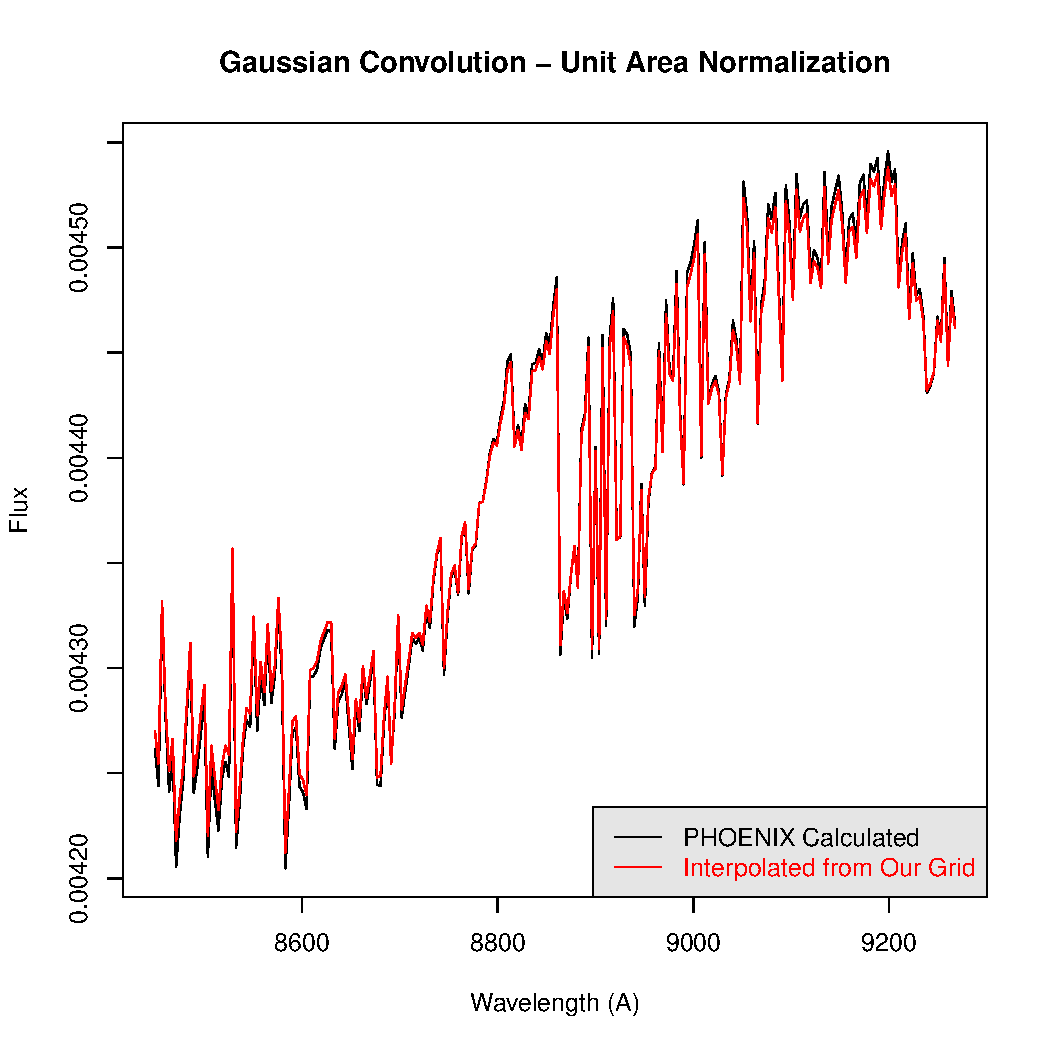
\includegraphics[width=6cm]{figs/intgrid4_gauss.pdf}
 \caption{Comparison between generated and interpollated spectrum}
 \label{fig:comp_gen_inter}
 \end{center}
\end {figure}

{
Then several other datasets can be created, by defining a mesh of 0.25 dex for 
both, log(gravity) and Metallicity. Temperature step was selected to be 50K, 
which produced 1329 spectra.
Then, another reinterpolation is produced, with a new 
step for temperature of 25K and 0.125 dex for log(gravity), 
keeping the metallicity step in 0.25 dex and producing 
a dataset with 25912 spectra. They can be used as needed for specific 
research pourposes. In spite of these, and in order to keep theirknowledge 
closer to the original BT-Settl source, most of the analyses have been 
performed with the original 535 spectra dataset.
}

{ The synthetic spectra are theoretical and they are noise free but it
  does not happen with real spectra.  To increase similarity with real
  observed spectra, gaussian noise has been added with two different
  Signal to Noise Ratios(SNR). The selected SNR were 10 and 50. {\bf
    Quizás deberíamos citar el trabajo de Ana como in preparation} }

\subsection{Feature definition and selection}
\label{subsec:FD}
{
It is well known that due to the special characteristics of 
physical parameters for these stars it is not easy to define 
suitable signal bands but it is even more complicated to identify 
the continuum chunks, were no signal shall be expected, because of the 
relative low temperatures they have and its impact on the emission 
rates at different wavelengths.
}

{
There are technical methodologies to identify suitable bands, as the one 
presented in (\cite{2013A&A...549A.129C}). %Cesetti ground base
In that case, bands I and K have been considered. His methodology is
mainly based on the sensitivity exhibited by different spectra through
different regions of the spectra. These observations were carried out by 
visual inspection.
}

{
The approach adopted in this paper was to estimate the three star relevant physical 
parameters ($T_{eff}$, Gravity and Metallicity) establishing a set of features, based on which
regression models could be useful for each of the physical parameters.

As the temperature is considered an strong parameter, it was used as known feature 
for the regression of the Gravity and Metalicity physical parameters.

The central contribution of this paper is the way to identify the most suitable
regions of spectrum (features) to be considered as signal providers 
but mainly the regions to be considered 
as candidates for being continuum for those signal regions.
It will be performed by means of artificial intelligence techniques.

These features consist of
a central bandpass covering the interesting lines and another bandpass
referring to the local continuum. Then, the feature can be written like 
Eq.~\eqref{eq:feature}.

\begin{equation}\label{eq:feature}
  F(i) =  \frac{ \int_{\lambda_{1s}(i)}^{\lambda_{2s}(i)} \left(f(\lambda)\right) d{\lambda}}
               { \int_{\lambda_{1c}(i)}^{\lambda_{2c}(i)} \left(f(\lambda)\right) d{\lambda}} 
               \quad \quad \forall i \in [1 \ldots N]
\end{equation}


where:
\begin{itemize}
 \item {N means the number of features to be considered, as decided by the researcher.}
 \item {$f(x)$ denotes the normalized flux spectra from the star.}
 \item {$(\lambda_{1s},\lambda_{2s})$ {\AA} accounts for the region of spectrum where the signal is considered. \quad \label{eq:cons1}}
 \item {$(\lambda_{1c},\lambda_{2c})$ {\AA} accounts for the region of spectrum where the continuum is considered.}
\end{itemize}

{
Now, the research question is how to identify 
$\{\lambda_{1s}(i),\lambda_{2s}(i), \lambda_{1c}(i),\lambda_{2c}(i)\}  \quad \forall i \in [1 \ldots N] $
in such a way they become useful to estimate the physical parameters.

Some constaints were estabished as designing of the selection process:

\begin{itemize}
 \item { $ \vert \lambda_{2k(i)} - \lambda_{1k(i)} \vert = 30 $ pixels of spectrum $ \quad \forall i \in [1 \ldots N]$ and $ k \in \{s,c\} $ .}
 \item { $ min ( \lambda_{1k(i)}, \lambda_{1k(j)} ) = 5 $ pixels of spectrum $ \quad \forall i,j \in [1 \ldots N] $ ; $ i \neq j $ and $ k \in \{s,c\} $ .}
 \item { $ \overline{\lambda_{2}(i)\lambda_{1}(i)}  \bigcap 
                      \overline{\lambda_{2c}(i)\lambda_{1c}(i)} = \emptyset \quad \forall i \in [1 \ldots N]$.}
\end{itemize}

which become a guarantee avoiding any overlap 
and a minimum size for both signal and continuum bandpasses.
}

{
Search for those features will depend on which specific physical parameter is 
under consideration but, the proposed methodology will look for those values 
trying to solve an optimization problem, which shall be the forecast capabilities
of one specific set of features, to be retained when it becomes bigger than 
a threshold.

To accomplish such optimization problem involving the selection of variable 
subsets, the use of the Genetic Algorithms technique was accepted. 
}

{ It was proposed to use the software tools R(\cite{R2013}).  There
  are different statistics to identify features that are
  differentially expressed between two or more groups of samples and
  then uses the most differentially expressed to construct a
  statistical model.  }

{ These methods have demonstrated to perform well, however, in some
  cases they can be ineffective regardless of the classification
  method used. An obvious conceptual limitation of univariate
  approaches is also the lack of consideration that features works in
  the contexts of interconnected pathways and therefore it is their
  behavior as a group that may be predictive of the phenotypic
  variables. Multivariate selection methods may seem to be more
  suitable for the analysis of data since variables are tested in
  combination to identify interactions between features. However, the
  extremely large number of models that can be constructed from
  different combination of thousands of features cannot be extensively
  evaluated using standard computational resources.  }

{ For the sake of simplicity let us define Genetic Algorithms (GAs)
  are variable search procedures that are based on the principle of
  evolution by natural selection. The procedure works by evolving sets
  of variables (chromosomes) that fit certain criteria from an initial
  random population via cycles of differential replication,
  recombination and mutation of the fittest chromosomes. The concept
  of using in-silico evolution for the solution of optimization
  problems has been introduced by John Holland in 1975
  (\cite{holland1975adaptation}). Although their application has been
  reasonably widespread (see Goldberg\textquoteright s book
  (\cite{goldberg1989genetic}), they became very popular only when
  sufficiently powerful computers became available.  }

{
The implementation of the GA follows the next steps:
\begin{itemize}
 \item [\textbf{Stage 1}:]{To produce the population of potential features (chromosomes).}
 \item [\textbf{Stage 2}:]{Each chromosome in the population is evaluated for its ability to
predict the group membership of each sample in the dataset (fitness function).}
 \item [\textbf{Stage 3}:]{Chromosome preselection, when a chromosome has 
 a score higher then a predefined value.}
 \item [\textbf{Stage 4}:]{The population of chromosomes is replicated. 
 Chromosomes with a higher fitness score will 
 generate a more numerous offspring.}
 \item [\textbf{Stage 5}:]{The genetic information contained in the replicated parent
chromosomes is combined through genetic crossover. Two randomly selected
parent chromosomes are used to create two new chromosomes.}
 \item [\textbf{Stage 6}:]{Mutations are then introduced in the chromosome randomly. 
 These mutations produce that new genes are used in chromosomes.
 Steps 5 and 6 are applied over the chromosomes establised at Step 4.}
  \item [\textbf{Stage 7}:]{This process is repeated from Stage 2 until 
  enough accuracy is obtained or the maximum of iterations is attained.}
\end{itemize}

The features were constructed as indicated above and named according
to the ordinal of the wavelength step both for signal and
continuum. The name includes also the number of ofset induced because
of the constraint \ref{eq:cons1}.  Polulation size was choosed as one
thousand individuals and accepted iterations were four thousand.
Three randomly started different repetions where produced bringing the
opportunity for enough variety and probabilities were established as
0.85 to corossover and 0.35 to mutation. The elitism was fixed to be
0.15.  Fitness for features were established as related to the Akaike
Criterion (-AIC) for linearity between the potential feature against
the physical parameter.  The most frequent and efficient features were
suggeswted as candidates to describe the behavior of specific physical
parameters.

From the implementation point of view a binarized codification was
selected in accordance to the naming convention and in order to speed
up the computation, a parallel implementation from a farm of fifteen
connected computers were used for each of the physical parameters.  }


{ The GA procedure provides us with a large collection of chromosomes.
  Although these are all potential solutions of the problem, it is not
  clear which one should be chosen for developing a model becoming for
  interpretation.  For this reason there is a need to develop a single
  model that is, to some extent, representative of the population. The
  simpler strategy to follow is to use the frequency of the chromosme
  in the population of chromosomes as criteria for inclusion in a
  forward selection strategy, however for this particular applciation,
  the choice was to include features based on their highest fitness.

After applying this technique the recommended features for temperature 
can be found in Table~\ref{tab:tab_NC_T}. 

\begin{table}
\begin{center}
\begin{tabular}{rrrrrrr}
  \hline
 & Signal From & Signal To & Continuum From & Continuum To & Fitness & Freq \\ 
  \hline
Feature 1 & 8376.10 & 8433.91 & 9346.13 & 9403.92 & -6693.10 & 319 \\ 
  Feature 2 & 8385.99 & 8443.94 & 9346.13 & 9403.92 & -6700.15 &   6 \\ 
  Feature 3 & 8195.96 & 8254.03 & 9386.01 & 9444.05 & -6887.55 &  44 \\ 
  Feature 4 & 8186.06 & 8243.98 & 9235.98 & 9294.01 & -7056.23 &  19 \\ 
  Feature 5 & 8406.00 & 8464.07 & 9515.96 & 9574.13 & -7068.86 &  34 \\ 
  Feature 6 & 9326.07 & 9384.15 & 8406.00 & 8464.07 & -7349.99 &  18 \\ 
  Feature 7 & 8496.05 & 8554.06 & 9576.03 & 9634.04 & -7505.21 &  38 \\ 
  Feature 8 & 9036.07 & 9094.04 & 9075.93 & 9133.98 & -7535.71 &  15 \\ 
  Feature 9 & 9135.89 & 9193.92 & 9085.96 & 9144.03 & -7622.16 &  27 \\ 
  Feature 10 & 9515.96 & 9574.13 & 8876.08 & 8934.03 & -7655.59 &   6 \\ 
  Feature 11 & 8716.00 & 8773.99 & 9025.93 & 9084.07 & -7703.40 &  77 \\ 
  Feature 12 & 9156.03 & 9214.07 & 8255.97 & 8314.06 & -7708.62 &  15 \\ 
  Feature 13 & 8266.11 & 8324.03 & 8235.96 & 8294.04 & -7856.20 &  30 \\ 
  Feature 14 & 8235.96 & 8294.04 & 8255.97 & 8314.06 & -7860.73 &  69 \\ 
  Feature 15 & 8705.93 & 8763.97 & 8886.00 & 8943.99 & -7919.62 &  27 \\ 
  Feature 16 & 8536.03 & 8594.06 & 8336.02 & 8394.08 & -7940.67 &  24 \\ 
  Feature 17 & 8605.97 & 8663.96 & 8346.02 & 8404.06 & -7953.63 &  59 \\ 
  Feature 18 & 8946.07 & 9004.01 & 8756.09 & 8814.06 & -8117.90 &  46 \\ 
  Feature 19 & 9135.89 & 9193.92 & 9485.83 & 9544.11 & -8211.98 &  36 \\ 
  Feature 20 & 8536.03 & 8594.06 & 8496.05 & 8554.06 & -8337.36 &  31 \\ 
   \hline
\end{tabular}
\caption {Recommended features and Continuum bandpass for predicting $ T_{eff} $ 
      by using BT\_Settl with SNR= $ {\infty} $ . 
      The Fitness and frequency of occurence are also included.} \label{tab:tab_NC_T} 
\end{center}
\end{table}

The authors have estimated the suggested features when theoretical BT\_Settl 
is noised with different SNR and following tables \ref{tab:tab_SNR10_T} 
and \ref{tab:tab_SNR50_T} sumarize the findings.


\begin{table}
\begin{center}
\begin{tabular}{rrrrrrr}
  \hline
 & Signal From & Signal To & Continuum From & Continuum To & Fitness & Freq \\ 
  \hline
Feature 1 & 8385.99 & 8443.94 & 9395.94 & 9454.03 & -6734.59 & 136 \\ 
  Feature 2 & 8186.06 & 8243.98 & 9536.15 & 9593.96 & -6857.65 &   7 \\ 
  Feature 3 & 8186.06 & 8243.98 & 9376.07 & 9433.92 & -6947.54 &   7 \\ 
  Feature 4 & 8286.01 & 8343.92 & 9206.05 & 9264.00 & -7123.10 &  10 \\ 
  Feature 5 & 8355.96 & 8414.03 & 9066.05 & 9124.05 & -7207.55 &  37 \\ 
  Feature 6 & 9276.00 & 9333.87 & 8415.91 & 8473.96 & -7436.13 &  32 \\ 
  Feature 7 & 8455.96 & 8513.93 & 9055.94 & 9114.07 & -7476.12 &  32 \\ 
  Feature 8 & 8616.00 & 8673.98 & 9576.03 & 9634.04 & -7491.24 &   6 \\ 
  Feature 9 & 8536.03 & 8594.06 & 9135.89 & 9193.92 & -7573.72 &  58 \\ 
  Feature 10 & 9395.94 & 9454.03 & 9356.05 & 9414.08 & -7586.78 &  45 \\ 
  Feature 11 & 9576.03 & 9634.04 & 9045.91 & 9103.99 & -7641.39 &  19 \\ 
  Feature 12 & 9066.05 & 9124.05 & 8166.02 & 8224.12 & -7642.28 &  15 \\ 
  Feature 13 & 9386.01 & 9444.05 & 9536.15 & 9593.96 & -7684.66 &   7 \\ 
  Feature 14 & 8616.00 & 8673.98 & 8756.09 & 8814.06 & -7686.46 &  17 \\ 
  Feature 15 & 9576.03 & 9634.04 & 8145.92 & 8204.03 & -7767.19 &  13 \\ 
  Feature 16 & 9466.08 & 9523.82 & 9036.07 & 9094.04 & -7772.45 &  37 \\ 
  Feature 17 & 9445.97 & 9504.01 & 9545.87 & 9604.02 & -7830.60 &  35 \\ 
  Feature 18 & 8286.01 & 8343.92 & 8486.02 & 8544.05 & -7863.15 &  49 \\ 
  Feature 19 & 9186.03 & 9244.04 & 9135.89 & 9193.92 & -7884.30 &  13 \\ 
  Feature 20 & 9306.03 & 9363.93 & 8745.93 & 8803.93 & -8020.27 &  56 \\ 
  Feature 21 & 8305.94 & 8364.04 & 8215.93 & 8273.93 & -8068.94 &  27 \\ 
  Feature 22 & 8186.06 & 8243.98 & 8326.00 & 8383.94 & -8288.51 &   6 \\ 
  Feature 23 & 8786.02 & 8844.10 & 8886.00 & 8943.99 & -8305.69 &  12 \\ 
  Feature 24 & 8855.96 & 8913.97 & 8366.04 & 8424.04 & -8309.97 &   7 \\ 
  Feature 25 & 8235.96 & 8294.04 & 8795.98 & 8853.95 & -8312.84 &  17 \\ 
  Feature 26 & 8786.02 & 8844.10 & 8385.99 & 8443.94 & -8318.31 &  59 \\ 
  Feature 27 & 8186.06 & 8243.98 & 8795.98 & 8853.95 & -8324.63 &   6 \\ 
  Feature 28 & 8855.96 & 8913.97 & 8286.01 & 8343.92 & -8334.47 &  34 \\ 
   \hline
\end{tabular}
\caption {Recommended features and Continuum bandpass for predicting $ T_{eff} $ 
      by using BT\_Settl with SNR= $ 10 $ . 
      The Fitness and frequency of occurence are also included.} \label{tab:tab_SNR10_T} 
\end{center}
\end{table}


\begin{table}
\begin{center}
\begin{tabular}{rrrrrrr}
  \hline
 & Signal From & Signal To & Continuum From & Continuum To & Fitness & Freq \\ 
  \hline
Feature 1 & 8376.10 & 8433.91 & 9346.13 & 9403.92 & -6693.10 & 545 \\ 
  Feature 2 & 8286.01 & 8343.92 & 9186.03 & 9244.04 & -7250.83 &  17 \\ 
  Feature 3 & 8476.01 & 8534.03 & 9525.89 & 9584.05 & -7392.49 &  38 \\ 
  Feature 4 & 9276.00 & 9333.87 & 9425.95 & 9484.00 & -7578.17 &  19 \\ 
  Feature 5 & 9555.93 & 9614.06 & 8886.00 & 8943.99 & -7652.77 &  54 \\ 
  Feature 6 & 9536.15 & 9593.96 & 8195.96 & 8254.03 & -7665.45 &  37 \\ 
  Feature 7 & 8515.98 & 8573.99 & 8936.05 & 8994.03 & -7687.69 &  19 \\ 
  Feature 8 & 8605.97 & 8663.96 & 8846.03 & 8904.03 & -7819.75 &  41 \\ 
  Feature 9 & 9285.87 & 9344.05 & 9096.06 & 9154.07 & -7841.07 &  12 \\ 
  Feature 10 & 8775.95 & 8833.94 & 9036.07 & 9094.04 & -7846.05 &  47 \\ 
  Feature 11 & 9346.13 & 9403.92 & 8826.01 & 8883.94 & -7873.89 &  16 \\ 
  Feature 12 & 9566.01 & 9623.96 & 9105.87 & 9163.91 & -7967.65 &   7 \\ 
  Feature 13 & 9566.01 & 9623.96 & 9536.15 & 9593.96 & -7998.01 &  42 \\ 
  Feature 14 & 8536.03 & 8594.06 & 8385.99 & 8443.94 & -8055.85 &  39 \\ 
  Feature 15 & 8846.03 & 8904.03 & 8395.98 & 8453.99 & -8118.20 &  16 \\ 
  Feature 16 & 9135.89 & 9193.92 & 9455.86 & 9514.14 & -8123.39 &  38 \\ 
  Feature 17 & 8515.98 & 8573.99 & 8415.91 & 8473.96 & -8233.55 &  42 \\ 
  Feature 18 & 8235.96 & 8294.04 & 8886.00 & 8943.99 & -8316.98 &   6 \\ 
  Feature 19 & 8366.04 & 8424.04 & 8195.96 & 8254.03 & -8320.41 &  17 \\ 
  Feature 20 & 8305.94 & 8364.04 & 8846.03 & 8904.03 & -8327.38 &  37 \\ 
  Feature 21 & 8795.98 & 8853.95 & 8835.93 & 8893.97 & -8327.43 &  35 \\ 
  Feature 22 & 8835.93 & 8893.97 & 8795.98 & 8853.95 & -8336.98 &  20 \\ 
   \hline
\end{tabular}
\caption {Recommended features and Continuum bandpass for predicting $ T_{eff} $ 
      by using BT\_Settl with SNR= $ 50 $ . 
      The Fitness and frequency of occurence are also included.} \label{tab:tab_SNR50_T} 
\end{center}
\end{table}


As in (\cite{2013A&A...549A.129C}) the authors provided their 
best estimation for suitable features, our interest is also to verify how
good it becomes in our particular case, as 
it can be an inderect assessment for the quality of the GA based recommendation. 

As a matter of reference the 
bandpass presented in Table ~\ref{tab:tab_cesetti} exploits the following bandpass:

\begin{table}
\begin{center}
\begin{tabular}{rrrrrrr}
  \hline
 & Signal\_from & Signal\_To & Cont1\_From & Cont1\_To & Cont2\_From & Cont2\_To \\ 
  \hline
Pa1 & 8461 & 8474 & 8474 & 8484 & 8563 & 8577 \\ 
  Ca1 & 8484 & 8513 & 8474 & 8484 & 8563 & 8577 \\ 
  Ca2 & 8522 & 8562  & 8474 & 8484 & 8563 & 8577 \\ 
  Pa2 & 8577 & 8619 & 8563 & 8577 & 8619 & 8642 \\ 
  Ca3 & 8642 & 8682 & 8619 & 8642 & 8700 & 8725 \\ 
  Pa3 & 8730 & 8772 & 8700 & 8725 & 8776 & 8792 \\ 
  Mg & 8802 & 8811 & 8776 & 8792 & 8815 & 8850 \\ 
  Pa4 & 8850 & 8890 & 8815 & 8850 & 8890 & 8900 \\ 
  Pa5 & 9000 & 9030 & 8983 & 8998 & 9040 & 9050 \\
  FeClTi & 9080 & 9100 & 9040 & 9050 & 9125 & 9135 \\
  Pa6 & 9217 & 9255 & 9152 & 9165 & 9265 & 9275 \\
   \hline
\end{tabular}
\caption {Recommended features and Continuum bandpass recommended in 
   \cite{2013A&A...549A.129C} as relevant for temperature inside Band I}
   \label{tab:tab_cesetti} 
\end{center}
\end{table}


In regards with the Gravity, the GA recommends the features 
presentend in Table~\ref{tab:tab_SNRoo_G} for the pure synthetic signal.

\begin{table}
\begin{center}
\begin{tabular}{rrrrrrr}
  \hline
 & Signal From & Signal To & Continuum From & Continuum To & Fitness & Freq \\ 
  \hline
Feature 1 & 8176.03 & 8234.13 & 8295.99 & 8353.99 & -1244.00 & 278 \\ 
  Feature 2 & 8176.03 & 8234.13 & 8955.88 & 9013.95 & -1506.62 &   8 \\ 
  Feature 3 & 8636.06 & 8694.06 & 8536.03 & 8594.06 & -1515.42 &  14 \\ 
  Feature 4 & 8486.02 & 8544.05 & 8985.93 & 9043.98 & -1519.48 &  50 \\ 
  Feature 5 & 8496.05 & 8554.06 & 9436.02 & 9493.86 & -1520.16 &   6 \\ 
  Feature 6 & 9085.96 & 9144.03 & 9276.00 & 9333.87 & -1522.24 &  15 \\ 
  Feature 7 & 9315.88 & 9374.02 & 9566.01 & 9623.96 & -1524.35 &  11 \\ 
  Feature 8 & 8985.93 & 9043.98 & 9285.87 & 9344.05 & -1527.06 &   9 \\ 
  Feature 9 & 8245.98 & 8304.08 & 9006.05 & 9064.02 & -1529.28 &  29 \\ 
  Feature 10 & 9156.03 & 9214.07 & 8376.10 & 8433.91 & -1532.13 &  17 \\ 
  Feature 11 & 8215.93 & 8273.93 & 8596.11 & 8654.10 & -1534.68 &  21 \\ 
  Feature 12 & 9276.00 & 9333.87 & 9395.94 & 9454.03 & -1537.74 &   6 \\ 
  Feature 13 & 8235.96 & 8294.04 & 8205.98 & 8263.96 & -1540.04 &  33 \\ 
  Feature 14 & 9576.03 & 9634.04 & 8145.92 & 8204.03 & -1541.89 &  61 \\ 
   \hline
\end{tabular}
\caption {Recommended features and Continuum bandpass for predicting $log(g)$ 
      by using BT\_Settl with SNR= $ \infty $ . 
      The Fitness and frequency of occurence are also included.} \label{tab:tab_SNRoo_G} 
\end{center}
\end{table}

The authors have produced the estimations for different SNR again 
as depicted in the tables \ref{tab:tab_SNR10_G} and \ref{tab:tab_SNR50_G}.

\begin{table}
\begin{center}
\begin{tabular}{rrrrrrr}
  \hline
 & Signal From & Signal To & Continuum From & Continuum To & Fitness & Freq \\ 
  \hline
Feature 1 & 8176.03 & 8234.13 & 8295.99 & 8353.99 & -1244.00 & 248 \\ 
  Feature 2 & 8176.03 & 8234.13 & 8305.94 & 8364.04 & -1252.85 &  16 \\ 
  Feature 3 & 8176.03 & 8234.13 & 8266.11 & 8324.03 & -1264.86 &   9 \\ 
  Feature 4 & 8556.06 & 8614.04 & 8716.00 & 8773.99 & -1489.47 &  33 \\ 
  Feature 5 & 8536.03 & 8594.06 & 9096.06 & 9154.07 & -1517.47 &  18 \\ 
  Feature 6 & 9135.89 & 9193.92 & 9536.15 & 9593.96 & -1517.92 &  38 \\ 
  Feature 7 & 8446.03 & 8503.94 & 9135.89 & 9193.92 & -1524.31 &   7 \\ 
  Feature 8 & 8446.03 & 8503.94 & 9306.03 & 9363.93 & -1525.64 &   8 \\ 
  Feature 9 & 9506.13 & 9563.85 & 9306.03 & 9363.93 & -1530.90 &  31 \\ 
  Feature 10 & 8925.98 & 8983.96 & 9485.83 & 9544.11 & -1534.00 &   7 \\ 
  Feature 11 & 9455.86 & 9514.14 & 9265.98 & 9323.99 & -1534.03 &  13 \\ 
  Feature 12 & 8355.96 & 8414.03 & 8406.00 & 8464.07 & -1534.04 &   8 \\ 
  Feature 13 & 9216.01 & 9274.05 & 8336.02 & 8394.08 & -1534.62 &   9 \\ 
  Feature 14 & 8925.98 & 8983.96 & 9436.02 & 9493.86 & -1535.91 &  27 \\ 
  Feature 15 & 9295.98 & 9354.08 & 8596.11 & 8654.10 & -1537.61 &  37 \\ 
  Feature 16 & 9255.86 & 9314.01 & 9365.95 & 9424.02 & -1538.41 &   8 \\ 
  Feature 17 & 8955.88 & 9013.95 & 9265.98 & 9323.99 & -1540.02 &  36 \\ 
  Feature 18 & 8566.08 & 8624.07 & 8585.96 & 8643.95 & -1540.09 &  49 \\ 
  Feature 19 & 9576.03 & 9634.04 & 9085.96 & 9144.03 & -1540.34 &  13 \\ 
  Feature 20 & 8446.03 & 8503.94 & 8665.99 & 8723.96 & -1541.80 &   7 \\ 
  Feature 21 & 8446.03 & 8503.94 & 8556.06 & 8614.04 & -1542.23 &  38 \\ 
  Feature 22 & 8726.06 & 8784.07 & 8315.97 & 8374.00 & -1542.31 &  20 \\ 
   \hline
\end{tabular}
\caption {Recommended features and Continuum bandpass for predicting $log(g)$ 
      by using BT\_Settl with SNR= $ 10 $ . 
      The Fitness and frequency of occurence are also included.} \label{tab:tab_SNR10_G} 
\end{center}
\end{table}

\begin{table}
\begin{center}
\begin{tabular}{rrrrrrr}
  \hline
 & Signal From & Signal To & Continuum From & Continuum To & Fitness & Freq \\ 
  \hline
Feature 1 & 8176.03 & 8234.13 & 8205.98 & 8263.96 & -1320.54 &  50 \\ 
  Feature 2 & 8415.91 & 8473.96 & 8166.02 & 8224.12 & -1400.77 &  10 \\ 
  Feature 3 & 8645.93 & 8703.94 & 8665.99 & 8723.96 & -1422.86 &   8 \\ 
  Feature 4 & 8515.98 & 8573.99 & 8205.98 & 8263.96 & -1504.27 &   9 \\ 
  Feature 5 & 9425.95 & 9484.00 & 9146.00 & 9204.05 & -1512.67 &  13 \\ 
  Feature 6 & 8486.02 & 8544.05 & 8936.05 & 8994.03 & -1517.66 &  10 \\ 
  Feature 7 & 8476.01 & 8534.03 & 8976.09 & 9034.00 & -1522.11 &   7 \\ 
  Feature 8 & 8446.03 & 8503.94 & 9455.86 & 9514.14 & -1526.30 &  15 \\ 
  Feature 9 & 9156.03 & 9214.07 & 8346.02 & 8404.06 & -1529.63 &   9 \\ 
  Feature 10 & 9636.16 & 9693.91 & 8215.93 & 8273.93 & -1531.01 &   9 \\ 
  Feature 11 & 9135.89 & 9193.92 & 8385.99 & 8443.94 & -1531.25 &   9 \\ 
  Feature 12 & 8865.98 & 8923.94 & 9536.15 & 9593.96 & -1532.35 &   8 \\ 
  Feature 13 & 8665.99 & 8723.96 & 8685.95 & 8744.09 & -1532.53 &  21 \\ 
  Feature 14 & 9126.00 & 9184.09 & 8215.93 & 8273.93 & -1533.15 &  10 \\ 
  Feature 15 & 9525.89 & 9584.05 & 8355.96 & 8414.03 & -1534.59 &  17 \\ 
  Feature 16 & 8616.00 & 8673.98 & 9406.09 & 9463.96 & -1534.81 &   9 \\ 
  Feature 17 & 8626.02 & 8683.99 & 9335.79 & 9393.93 & -1534.98 &   8 \\ 
  Feature 18 & 8305.94 & 8364.04 & 8286.01 & 8343.92 & -1535.35 &  13 \\ 
  Feature 19 & 8685.95 & 8744.09 & 9096.06 & 9154.07 & -1535.57 &  19 \\ 
  Feature 20 & 8636.06 & 8694.06 & 8235.96 & 8294.04 & -1536.95 &  12 \\ 
  Feature 21 & 9395.94 & 9454.03 & 8826.01 & 8883.94 & -1539.98 &   6 \\ 
  Feature 22 & 8195.96 & 8254.03 & 9115.99 & 9174.04 & -1540.19 &  15 \\ 
  Feature 23 & 8786.02 & 8844.10 & 9235.98 & 9294.01 & -1542.00 &  10 \\  
   \hline
\end{tabular}
\caption {Recommended features and Continuum bandpass for predicting $log(g)$ 
      by using BT\_Settl with SNR= $ 50 $ . 
      The Fitness and frequency of occurence are also included.} \label{tab:tab_SNR50_G} 
\end{center}
\end{table}

Finally, features suggested for metallicity 
can be found in Table~\ref{tab:tab_SNRoo_M}.

\begin{table}
\begin{center}
\begin{tabular}{rrrrrrr}
  \hline
 & Signal From & Signal To & Continuum From & Continuum To & Fitness & Freq \\ 
  \hline
Feature 1 & 9085.96 & 9144.03 & 9445.97 & 9504.01  & -1146.72 & 348 \\ 
  Feature 2 & 9445.97 & 9504.01 & 9085.96 & 9144.03 & -1150.63 &  24 \\ 
  Feature 3 & 8556.06 & 8614.04 & 9135.89 & 9193.92 & -1209.47 &  11 \\ 
  Feature 4 & 9096.06 & 9154.07 & 8466.08 & 8523.98 & -1271.45 &   8 \\ 
  Feature 5 & 9045.91 & 9103.99 & 8525.91 & 8583.93 & -1276.04 &   5 \\  
   \hline
\end{tabular}
\caption {Recommended features and Continuum bandpass for predicting $Metallicity$ 
     by using BT\_Settl with SNR= $ \infty $ . 
      The Fitness and frequency of occurence are also included.} \label{tab:tab_SNRoo_M} 
\end{center}
\end{table}

And when different SNR are considered, the suggested features can be found in 
tables \ref{tab:tab_SNR10_M} and \ref{tab:tab_SNR50_M}

\begin{table}
\begin{center}
\begin{tabular}{rrrrrrr}
  \hline
 & Signal From & Signal To & Continuum From & Continuum To & Fitness & Freq \\ 
  \hline
Feature 1 & 9476.15 & 9534.00 & 9576.03 & 9634.04 & -1199.37 &  17 \\ 
  Feature 2 & 8466.08 & 8523.98 & 9146.00 & 9204.05 & -1207.84 & 189 \\ 
  Feature 3 & 8466.08 & 8523.98 & 9156.03 & 9214.07 & -1208.98 &  10 \\ 
  Feature 4 & 9466.08 & 9523.82 & 9416.04 & 9474.02 & -1220.23 &  12 \\ 
  Feature 5 & 9335.79 & 9393.93 & 9186.03 & 9244.04 & -1225.37 &  26 \\ 
  Feature 6 & 8466.08 & 8523.98 & 8936.05 & 8994.03 & -1230.60 &   8 \\ 
  Feature 7 & 9255.86 & 9314.01 & 9545.87 & 9604.02 & -1239.94 &  39 \\ 
  Feature 8 & 9285.87 & 9344.05 & 9495.98 & 9553.95 & -1249.38 &   7 \\ 
  Feature 9 & 9576.03 & 9634.04 & 8855.96 & 8913.97 & -1254.27 &   6 \\ 
  Feature 10 & 9285.87 & 9344.05 & 8505.89 & 8563.93 & -1255.30 &   7 \\ 
  Feature 11 & 9285.87 & 9344.05 & 9455.86 & 9514.14 & -1256.35 &  84 \\ 
  Feature 12 & 9636.16 & 9693.91 & 8245.98 & 8304.08 & -1258.18 &   6 \\ 
  Feature 13 & 9525.89 & 9584.05 & 9285.87 & 9344.05 & -1267.30 &  27 \\ 
  Feature 14 & 9545.87 & 9604.02 & 8826.01 & 8883.94 & -1269.76 &  34 \\ 
  Feature 15 & 9096.06 & 9154.07 & 8255.97 & 8314.06 & -1270.05 &   6 \\ 
  Feature 16 & 8286.01 & 8343.92 & 9235.98 & 9294.01 & -1270.11 &   6 \\ 
  Feature 17 & 8685.95 & 8744.09 & 8286.01 & 8343.92 & -1270.29 &  16 \\ 
  Feature 18 & 8775.95 & 8833.94 & 8556.06 & 8614.04 & -1271.08 &   6 \\ 
  Feature 19 & 9096.06 & 9154.07 & 9436.02 & 9493.86 & -1272.52 &  40 \\ 
  Feature 20 & 9485.83 & 9544.11 & 8336.02 & 8394.08 & -1272.86 &  31 \\ 
  Feature 21 & 8406.00 & 8464.07 & 9306.03 & 9363.93 & -1280.13 &  46 \\ 
  Feature 22 & 9045.91 & 9103.99 & 8665.99 & 8723.96 & -1294.98 &   6 \\ 
  Feature 23 & 8305.94 & 8364.04 & 8835.93 & 8893.97 & -1347.20 & 113 \\ 
  Feature 24 & 8385.99 & 8443.94 & 8205.98 & 8263.96 & -1348.16 &   9 \\ 
  Feature 25 & 8765.97 & 8823.95 & 8395.98 & 8453.99 & -1350.18 &  17 \\ 
   \hline
\end{tabular}
\caption {Recommended features and Continuum bandpass for predicting $Metallicity$ 
     by using BT\_Settl with SNR= $ 10 $ . 
      The Fitness and frequency of occurence are also included.} \label{tab:tab_SNR10_M} 
\end{center}
\end{table}

\begin{table}
\begin{center}
\begin{tabular}{rrrrrrr}
  \hline
 & Signal From & Signal To & Continuum From & Continuum To & Fitness & Freq \\ 
  \hline
Feature 1 & 9085.96 & 9144.03 & 9445.97 & 9504.01  & -1146.72 & 177 \\ 
  Feature 2 & 9445.97 & 9504.01 & 9085.96 & 9144.03 & -1150.63 &  5 \\ 
  Feature 3 & 8556.06 & 8614.04 & 9135.89 & 9193.92 & -1209.47 &  6 \\ 
  Feature 4 & 9096.06 & 9154.07 & 8466.08 & 8523.98 & -1271.45 &   6 \\ 
  Feature 5 & 9045.91 & 9103.99 & 8525.91 & 8583.93 & -1276.04 &   5 \\  
   \hline
\end{tabular}
\caption {Recommended features and Continuum bandpass for predicting $Metallicity$ 
     by using BT\_Settl with SNR= $ 50 $ . 
      The Fitness and frequency of occurence are also included.} \label{tab:tab_SNR50_M} 
\end{center}
\end{table}
  
  
}
